\documentclass{beamer}

\usepackage{times}

\usepackage{hyperref}

\hypersetup{
  urlcolor=blue,
  linkcolor=blue,
  colorlinks=true
}

\usepackage{listings}
\lstset{frame=none, showstringspaces=false, basicstyle=\ttfamily\bfseries\footnotesize,
  xleftmargin=-8mm,language=Haskell,breaklines=true}

\title {Sustainable Software via Generation}

\author{\textbf{Spencer Smith} and Jacques Carette}

\institute[McMaster University]
{
  Computing and Software Department\\
  Faculty of Engineering\\
  McMaster University
}

\date {BRIC 2021, Booth Resource and Innovation Cluster, First Annual Symposium:
  July 28, 2021}

\subject{research software, software engineering, software
  quality, code and artifact generation, software documentation}
% This is only inserted into the PDF information catalog. Can be left
% out. 

\beamertemplatenavigationsymbolsempty 

\begin{document}

%%%%%%%%%%%%%%%%%%%%%%%%%%%%%%%%%%%%%%

\begin{frame}[plain]

\titlepage

\end{frame}

%%%%%%%%%%%%%%%%%%%%%%%%%%%%%%%%%%%%%% 

\begin{frame}

\frametitle{Generate All Things with Drasil}

\begin{itemize}
\item \textbf{Goal} -- Improve quality of SCS
\item \textbf{Idea}
  \begin{itemize}
  \item Adapt ideas from SE
  \item Document requirements, design, verification, etc.
    \begin{itemize}
    \item Good -- improves quality
    \item Bad -- too much work, inevitable change, too hard to maintain
    \end{itemize}
  \end{itemize}
\item \textbf{Solution}
\begin{itemize}
\item Capture knowledge once
\item Generate all documentation and code
% \item Avoid duplication
% \item Traceability
% \item Reproducibility
\end{itemize}
\item \textbf{Implement Solution --
    \href{https://github.com/JacquesCarette/Drasil} {Drasil}}
  \begin{itemize}
  \item Facilitates change
  \item Traceability
  \item Reproducibility
  \item Sustainability
  \item Certification
  \item Captures best practices
  \end{itemize}
\end{itemize}

\end{frame}

%%%%%%%%%%%%%%%%%%%%%%%%%%%%%%%%%%%%%%

\begin{frame}

\frametitle{GlassBR}

\begin{columns}
\begin{column}{0.5\textwidth}
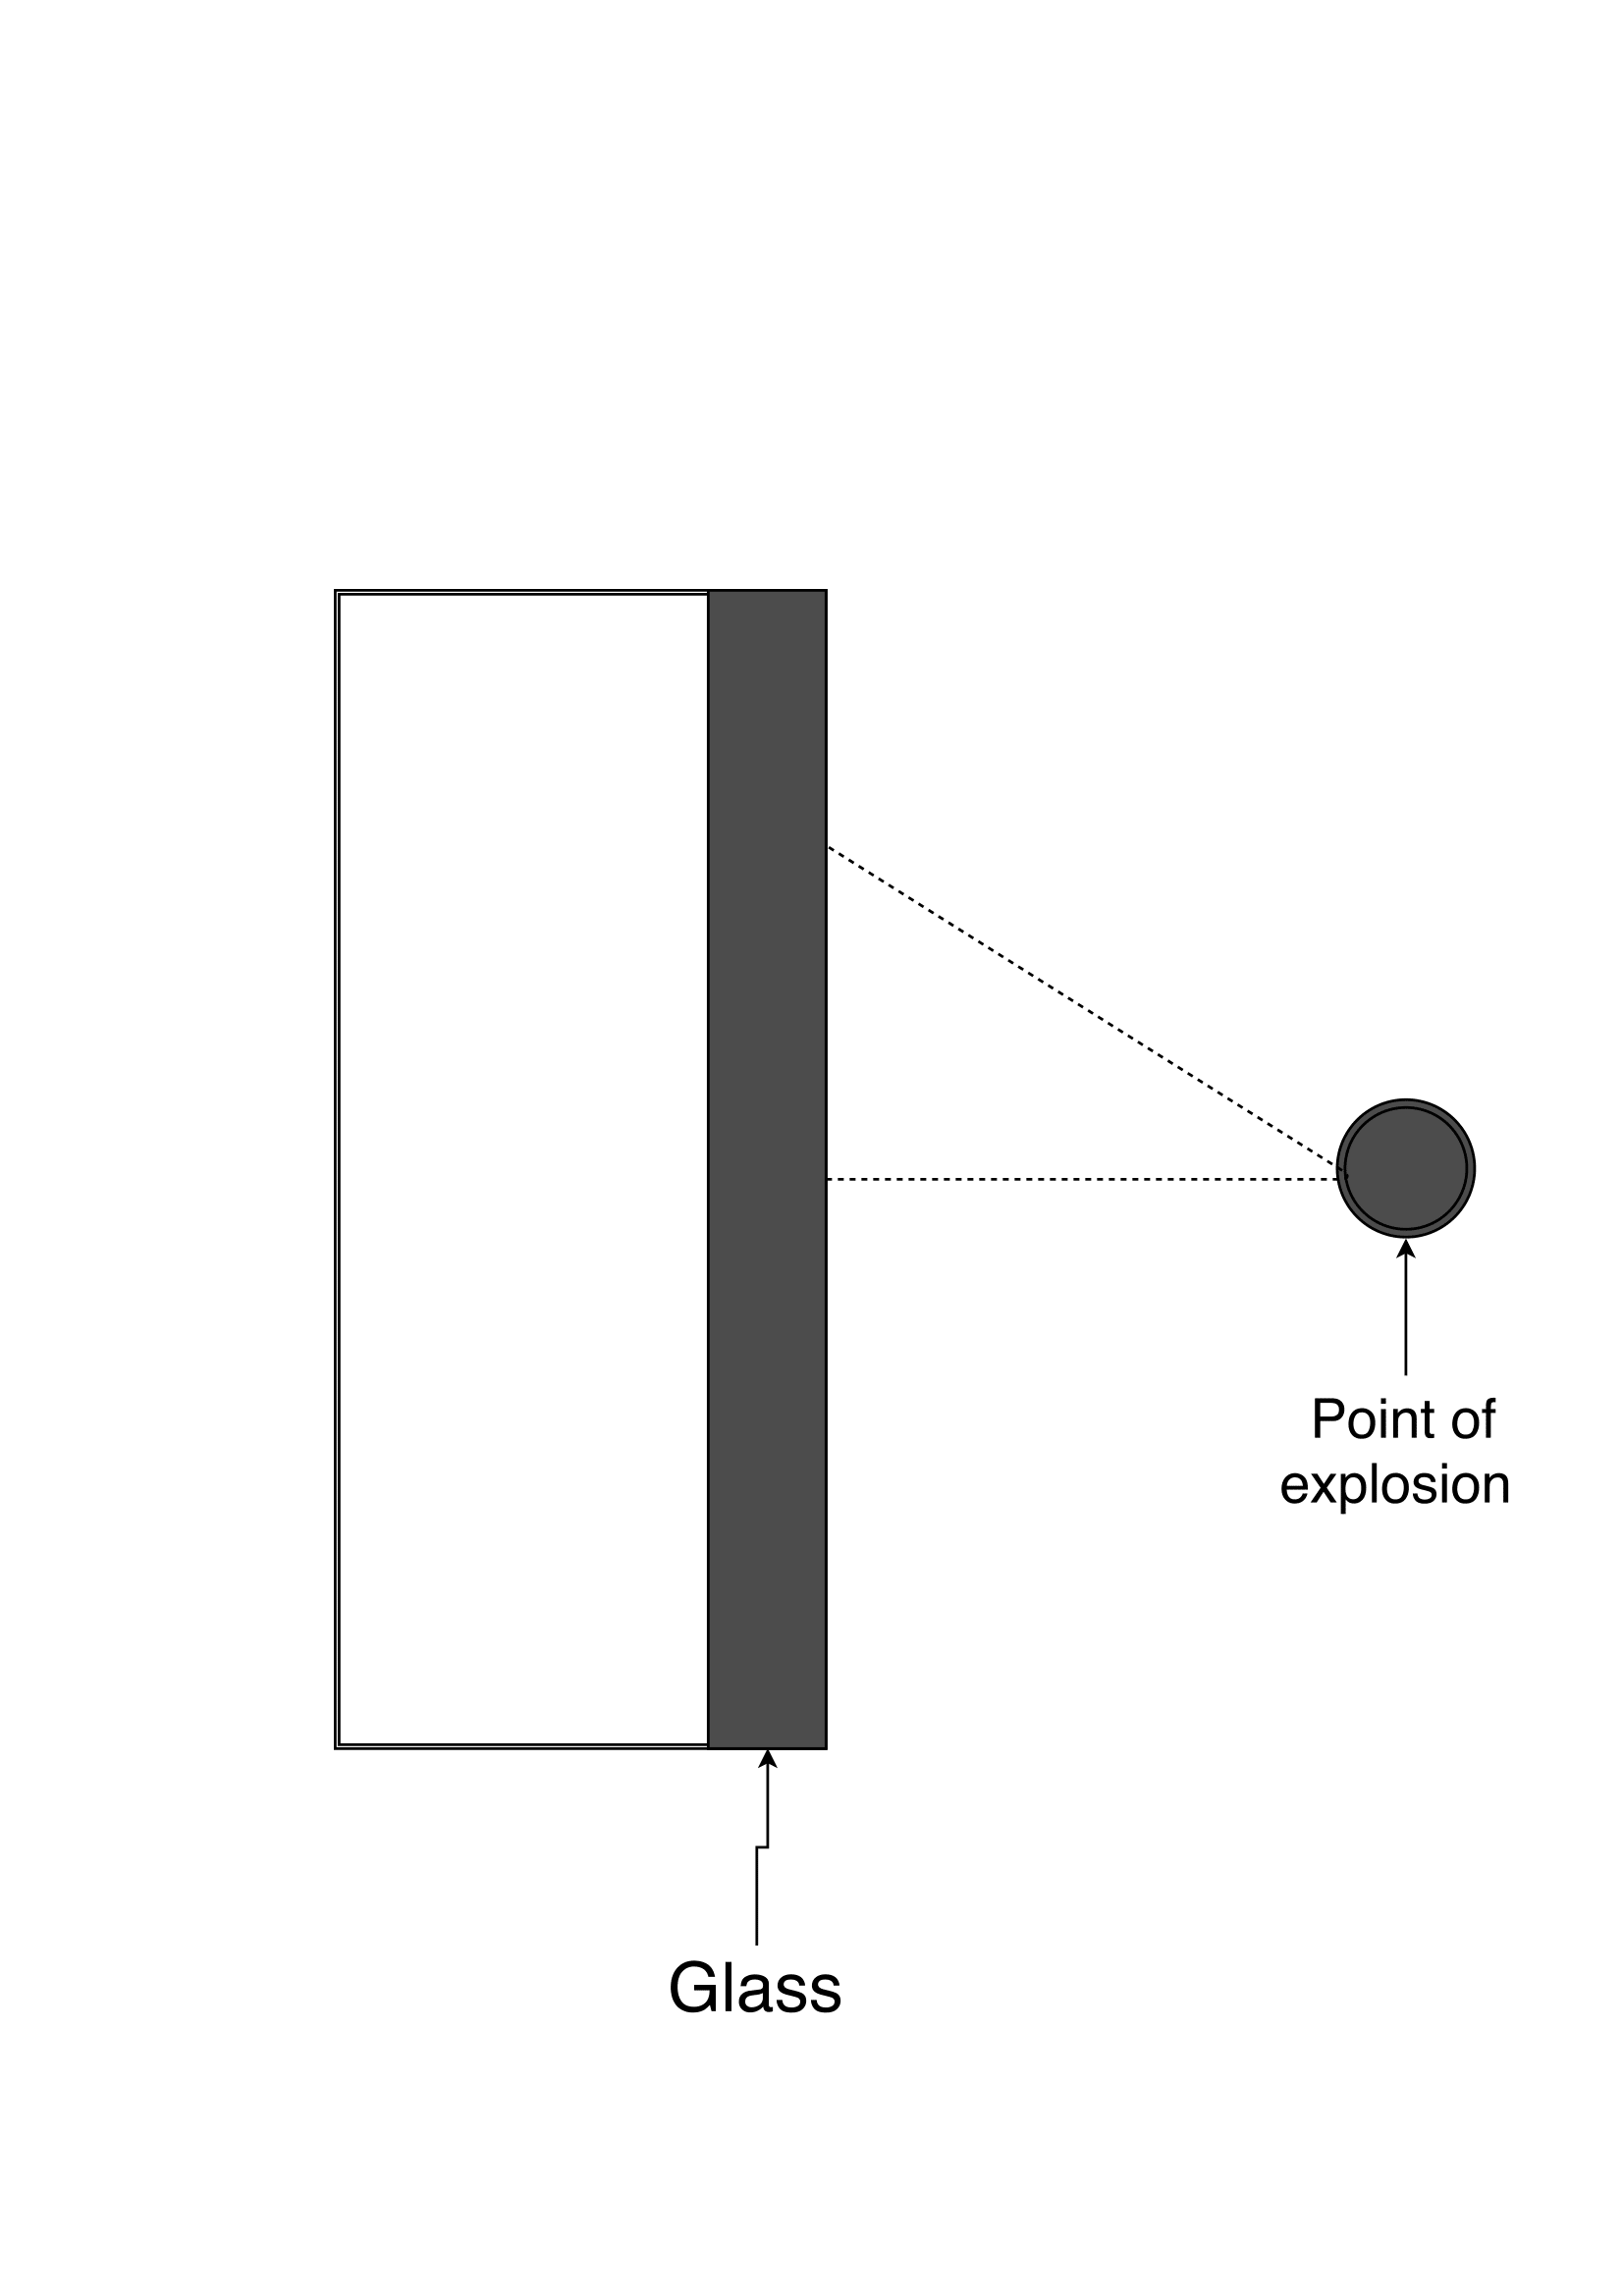
\includegraphics[width=1.0\textwidth]{../figures/physicalsystimage.png}
\end{column}
\begin{column}{0.5\textwidth}
Given

\begin{itemize}
\item dimensions of glass plane
\item glass type
\item explosion characteristics
\item tolerable breakage probability
\end{itemize}

Predict whether the glass will withstand the explosion

\end{column}
\end{columns}

\end{frame}

%%%%%%%%%%%%%%%%%%%%%%%%%%%%%%%%%%%%%%

\begin{frame}

%\frametitle{Input Knowledge}

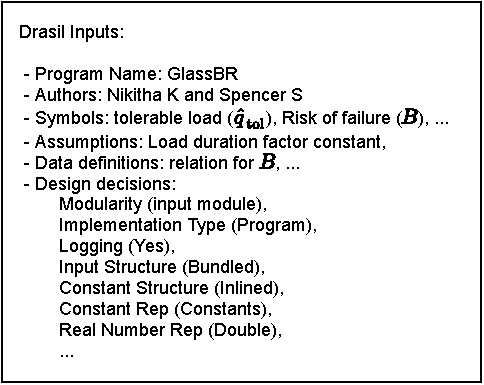
\includegraphics[width=0.95\textwidth]{../figures/DrasilInputs.pdf}

\end{frame}

%%%%%%%%%%%%%%%%%%%%%%%%%%%%%%%%%%%%%%

\begin{frame}

%\frametitle{Input Knowledge}

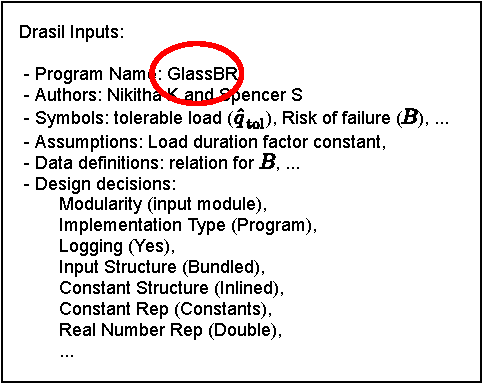
\includegraphics[width=0.95\textwidth]{../figures/InputsCircleGlassBR.pdf}

\end{frame}

%%%%%%%%%%%%%%%%%%%%%%%%%%%%%%%%%%%%%%

\begin{frame}

%\frametitle{Input Knowledge}

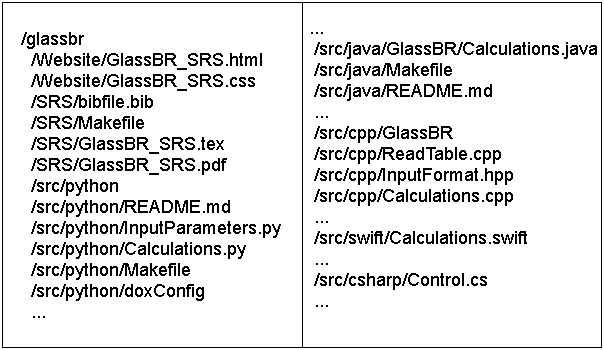
\includegraphics[width=1.05\textwidth]{../figures/FoldersFiles.pdf}

\end{frame}

%%%%%%%%%%%%%%%%%%%%%%%%%%%%%%%%%%%%%%

\begin{frame}

%\frametitle{Input Knowledge}

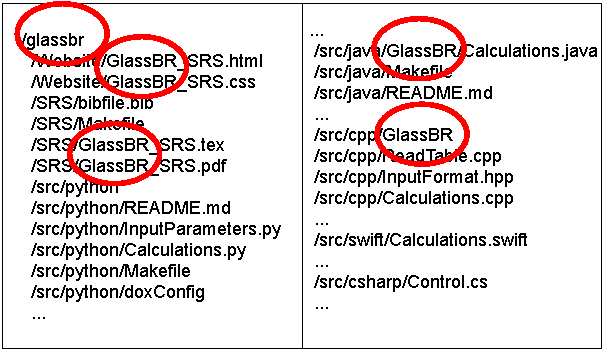
\includegraphics[width=1.05\textwidth]{../figures/FoldersFilesCircleGlassBR.pdf}

\end{frame}

%%%%%%%%%%%%%%%%%%%%%%%%%%%%%%%%%%%%%%

\begin{frame}

%\frametitle{Input Knowledge}

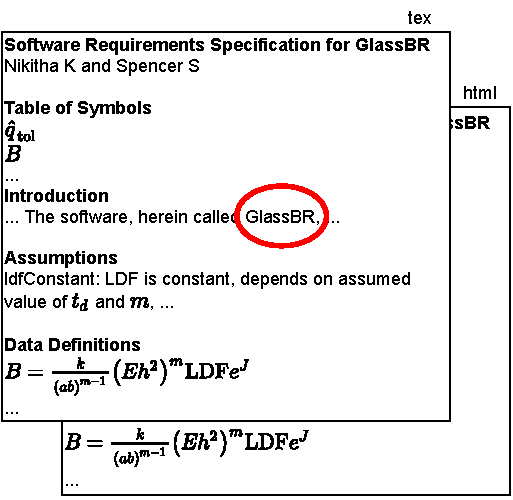
\includegraphics[width=1.05\textwidth]{../figures/SRSCircleGlassBR.pdf}

\end{frame}

%%%%%%%%%%%%%%%%%%%%%%%%%%%%%%%%%%%%%%

\begin{frame}

%\frametitle{Input Knowledge}

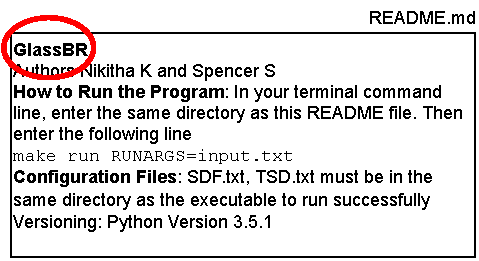
\includegraphics[width=1.05\textwidth]{../figures/READMECircleGlassBR.pdf}

\end{frame}

%%%%%%%%%%%%%%%%%%%%%%%%%%%%%%%%%%%%%%

\begin{frame}

%\frametitle{Input Knowledge}

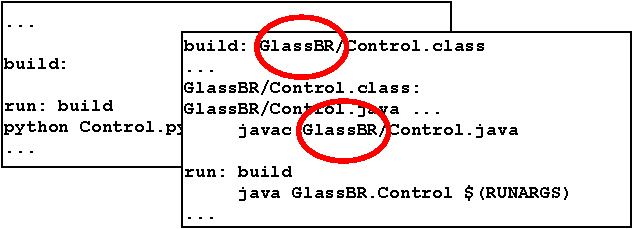
\includegraphics[width=1.05\textwidth]{../figures/MakefileCircleGlassBR.pdf}

\end{frame}

%%%%%%%%%%%%%%%%%%%%%%%%%%%%%%%%%%%%%%

\begin{frame}

%\frametitle{Input Knowledge}

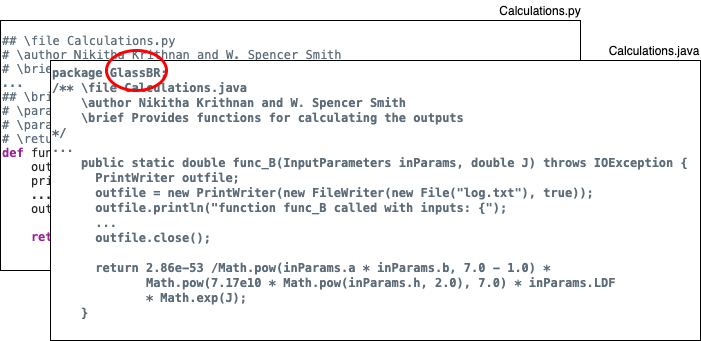
\includegraphics[width=1.05\textwidth]{../figures/CodeCircleGlassBR.png}

\end{frame}

%%%%%%%%%%%%%%%%%%%%%%%%%%%%%%%%%%%%%%

\begin{frame}

\frametitle{$J_{\mbox{tol}}$ in SRS.pdf}
\begin{center}
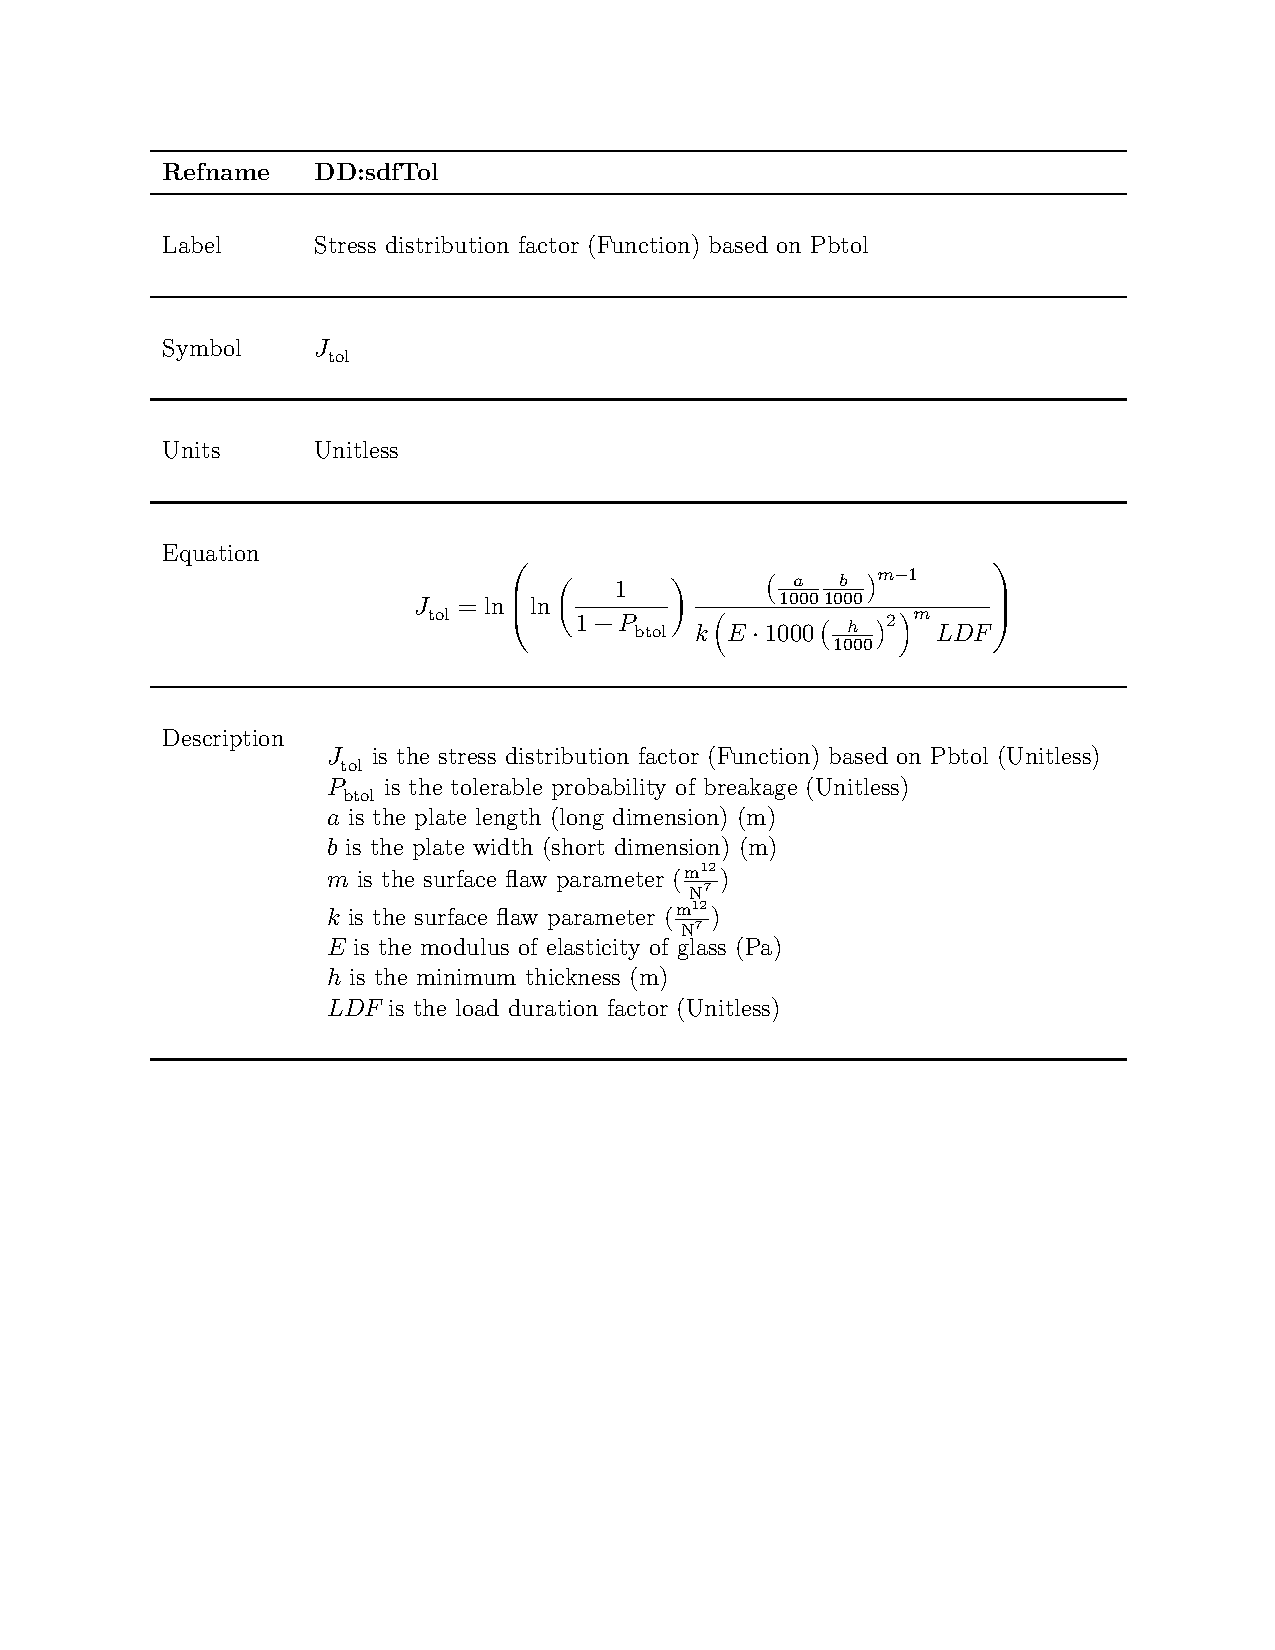
\includegraphics[width=0.9\textwidth]{../figures/Jtol_pdf.pdf}
\end{center}
\end{frame}

%%%%%%%%%%%%%%%%%%%%%%%%%%%%%%%%%%%%%

\begin{frame}[plain, fragile]

\frametitle{$J_{\mbox{tol}}$ in SRS.tex}
~\\
\begin{lstlisting}
...
Label & Stress distribution factor (Function) based on Pbtol
        
\\ \midrule \\
Symbol & ${J_{\text{tol}}}$
         
\\ \midrule \\
Units & Unitless
        
\\ \midrule \\
Equation & \begin{displaymath}
           {J_{\text{tol}}}=\ln\left(\ln\left(\frac{1}{1-{P_{\text{b}\text{tol}}}}\right) \frac{\left(\frac{a}{1000} \frac{b}{1000}\right)^{m-1}}{k \left(E\cdot{}1000 \left(\frac{h}{1000}\right)^{2}\right)^{m} LDF}\right)
           \end{displaymath}
\\ \midrule \\
Description & ...
\end{lstlisting}
\end{frame}

%%%%%%%%%%%%%%%%%%%%%%%%%%%%%%%%%%%%%%

\begin{frame}[plain, fragile]

\frametitle{$J_{\mbox{tol}}$ in SRS.html}

\begin{lstlisting}

...
<th>Equation</th>
<td>
\[{J_{\text{tol}}}=\ln\left(\ln\left(\frac{1}{1-{P_{\text{b}\text{tol}}}}\right) \frac{\left(\frac{a}{1000} \frac{b}{1000}\right)^{m-1}}{k \left(E\cdot{}1000 \left(\frac{h}{1000}\right)^{2}\right)^{m} LDF}\right)\]
</td>
...
\end{lstlisting}

\end{frame}
%%%%%%%%%%%%%%%%%%%%%%%%%%%%%%%%%%%%%

\begin{frame}[plain, fragile]

\frametitle{$J_{\mbox{tol}}$ in Python}

\begin{lstlisting}
## \brief Calculates stress distribution factor (Function) based on Pbtol
# \param inParams structure holding the input values
# \return stress distribution factor (Function) based on Pbtol
def func_J_tol(inParams):
    outfile = open("log.txt", "a")
    print("function func_J_tol called with inputs: {", file=outfile)
    print("  inParams = ", end="", file=outfile)
    print("Instance of InputParameters object", file=outfile)
    print("  }", file=outfile)
    outfile.close()
    
    return math.log(math.log(1.0 / (1.0 - inParams.P_btol)) * ((inParams.a / 1000.0 * (inParams.b / 1000.0)) ** (7.0 - 1.0) / (2.86e-53 * (7.17e10 * 1000.0 * (inParams.h / 1000.0) ** 2.0) ** 7.0 * inParams.LDF)))
\end{lstlisting}
\end{frame}

%%%%%%%%%%%%%%%%%%%%%%%%%%%%%%%%%%%%%%

\begin{frame}[plain, fragile]

\frametitle{$J_{\mbox{tol}}$ in Java}

\begin{lstlisting}
    /** \brief Calculates stress distribution factor (Function) based on Pbtol
        \param inParams structure holding the input values
        \return stress distribution factor (Function) based on Pbtol
    */
    public static double func_J_tol(InputParameters inParams) throws IOException {
        PrintWriter outfile;
        outfile = new PrintWriter(new FileWriter(new File("log.txt"), true));
        ...
        return Math.log(Math.log(1.0 / (1.0 - inParams.P_btol)) * (Math.pow(inParams.a / 1000.0 * (inParams.b / 1000.0), 7.0 - 1.0) / (2.86e-53 * Math.pow(7.17e10 * 1000.0 * Math.pow(inParams.h / 1000.0, 2.0), 7.0) * inParams.LDF)));
    }
\end{lstlisting}
\end{frame}

%%%%%%%%%%%%%%%%%%%%%%%%%%%%%%%%%%%%%%

\begin{frame}[plain, fragile]

\frametitle{$J_{\mbox{tol}}$ in Drasil (Haskell)}

\begin{lstlisting}

tolStrDisFacEq :: Expr
tolStrDisFacEq = ln (ln (recip_ (exactDbl 1 $- sy pbTol))
  `mulRe` (((sy plateLen $/ exactDbl 1000) `mulRe` (sy plateWidth $/ exactDbl 1000)) $^ (sy sflawParamM $- exactDbl 1) $/
    (sy sflawParamK `mulRe` ((sy modElas `mulRe` exactDbl 1000 `mulRe`
    square (sy minThick $/ exactDbl 1000)) $^ sy sflawParamM) `mulRe` sy lDurFac)))

\end{lstlisting}
\end{frame}

%%%%%%%%%%%%%%%%%%%%%%%%%%%%%%%%%%%%%%

\begin{frame}[plain, fragile]

\frametitle{$J_{\mbox{tol}}$ without Unit Conversion}

\begin{lstlisting}
tolStrDisFacEq :: Expr
tolStrDisFacEq = ln (ln (recip_ (exactDbl 1 $- sy pbTol))
  `mulRe` ((sy plateLen `mulRe` sy plateWidth) $^ (sy sflawParamM $- exactDbl 1) $/
    (sy sflawParamK `mulRe` ((sy modElas `mulRe`
    square (sy minThick)) $^ sy sflawParamM) `mulRe` sy lDurFac)))
\end{lstlisting}
\end{frame}

%%%%%%%%%%%%%%%%%%%%%%%%%%%%%%%%%%%%%%

\begin{frame}

%\frametitle{Input Knowledge}

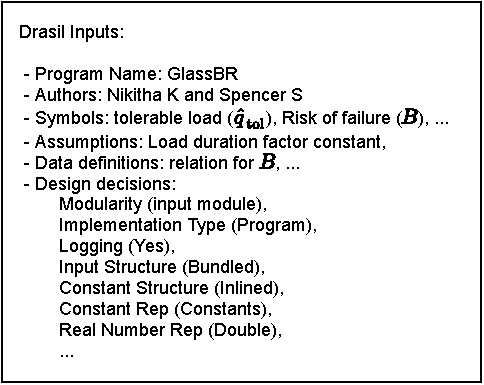
\includegraphics[width=0.95\textwidth]{../figures/DrasilInputs.pdf}

\end{frame}

%%%%%%%%%%%%%%%%%%%%%%%%%%%%%%%%%%%%%%

\begin{frame}

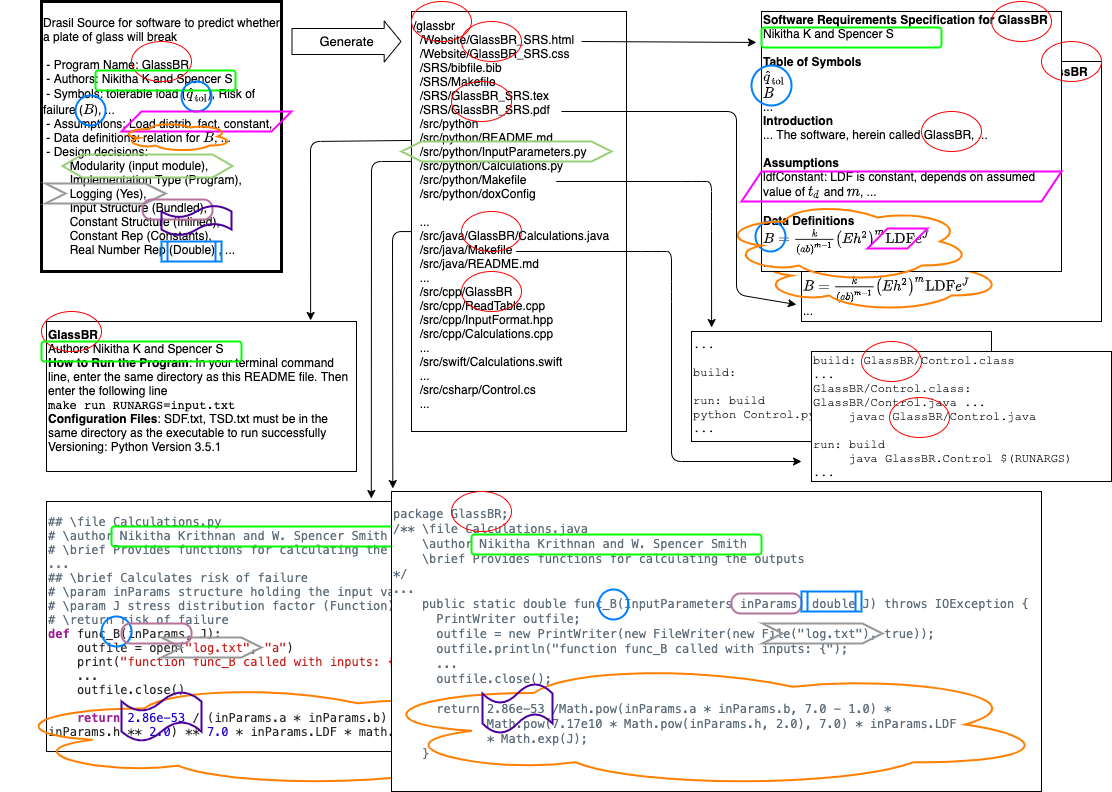
\includegraphics[width=1.0\textwidth]{../figures/DrasilSupportsChange.png}

\end{frame}

%%%%%%%%%%%%%%%%%%%%%%%%%%%%%%%%%%%%%%

\begin{frame}

\frametitle{Improve Software Qualities}

\begin{itemize}
\item Capture best practices
\item Explore alternatives  
\item Traceability
\item Reproducibility
\item Sustainability  
\item Certifiability
\item Reusability
\end{itemize}

\end{frame}

%%%%%%%%%%%%%%%%%%%%%%%%%%%%%%%%%%%%%%

\begin{frame}

\frametitle{Concluding Remarks}

\begin{itemize}
\item What Drasil can currently do
  \begin{itemize}
  \item Explicit relations, LHS = ...
  \item Linear first order ODEs
  \item Knowledge on rigid body mechanics, heat transfer
  \item SRS (LaTeX, html), code (Python, C++, C sharp, Java, Swift), README, Makefile
  \end{itemize}
\item Future additions
  \begin{itemize}
  \item More scientific knowledge: medical imaging, chemistry, more mechanics,
    etc.
  \item More computational knowledge: external libraries, linear systems
    solvers, higher order ODEs, root finding, etc.
  \item More document knowledge: Teaching lessons, academic papers, assurance
    cases, etc.
%  \item Sequences 
  \item Jupyter notebooks
  \item \href{https://github.com/JacquesCarette/Drasil/issues} {GitHub Issues}
  \end{itemize}

\end{itemize}

\end{frame}

%%%%%%%%%%%%%%%%%%%%%%%%%%%%%%%%%%%%%%

\end{document}